\documentclass[a4paper]{article}

%% Language and font encodings
\usepackage[english, russian]{babel}
\usepackage[utf8x]{inputenc}
\usepackage[T1]{fontenc}

%% Sets page size and margins
\usepackage[a4paper,top=3cm,bottom=2cm,left=3cm,right=3cm,marginparwidth=1.75cm]{geometry}

%% Useful packages
\usepackage{float}
\usepackage{amsmath}
\usepackage{graphicx}
\usepackage[colorinlistoftodos]{todonotes}
\usepackage[colorlinks=true, allcolors=blue]{hyperref}

\title{Работа 1.2 Изучение магнитного поля соленоида с помощью датчика Холла.}
\author{Дмитриева Ирина, 597 группа}
\date{}

\begin{document}
\maketitle

\section{Цель работы}
Изучение магнитного поля соленоида, магнитного поля постоянных магнитов, измерение индукции магнитного поля Земли.

\section{В работе используются}
соленоид, намотанный на полый цилиндрический каркас, набор из 10 постоянных магнитов в форме дисков ($d$ = 25 мм, $h$= 5 мм); 8 небольших одинаковых магнитиков (4х6х8 мм3, источник постоянного тока с встроенным амперметром, измеритель магнитной индукции Ш1-10 (магнитометр),измеритель магнитной индукции ATE–8702, весы, тонкая нить для изготовления крутильного маятника, секундомер, штангенциркуль, брусок из немагнитного материала 

\section{Теоретическая часть}
Магнитное поле порождается движущимися зарядами (токами). В соответствии с законом Био–Савара, линейный элемент тока $I dl$ на расстоянии $r$ создаёт магнитное поле с индукцией:
 \[B = \frac{\mu_{0}}{4 * \pi} I \frac{dl \times r}{r^{3}} \eqno(1)\]
    
Полное поле, вследствие принципа суперпозиции, определяется интегрированием выражения (1) по всем элементам тока
\[ B = \frac{\mu_{0}}{4\pi} \int  I \frac{dl \times r}{r^{3}} \eqno(2) \]

\textbf{Магнитное поле прямого провода.} 
Поле прямого бесконечного провода на расстоянии от него определяется выражением:
 \[B = \frac{\mu_{0}}{4 * \pi} \frac{2 I }{R} \eqno(3) \]
 
\textbf{Поле кругового тока.} 
 \[B = \frac{\mu_{0}}{4 * \pi} \frac{2 I S}{r^{3}} = \frac{\mu_{0}}{4 * \pi} \frac{2 P_{m}}{r^{3}} \eqno(4) \]
 
\textbf{Поле соленоида.} 
 \[B = \frac{\mu_{0}}{4 * \pi} I n \Omega \eqno(5) \],
 где $\Omega = \Omega_{1} - \Omega_{2}$ - телесный угол, под которым из точки наблюдения видна внутренняя поверхность соленоида, а $\Omega_{1}$ и $\Omega_{1}$ - телесные углы, под которыми видны из точки наблюдения торцы соленоида.
 
\textbf{Постоянные магниты.}
В произвольной точке А на оси диска магнитное поле

 \[B = \frac{\mu_{0}}{4 * \pi} 2 \pi p_{m} (cos\alpha - cos \beta) \eqno(6) \]
 Для точки O в центре торца: $cos \beta = 0$, а $cos \alpha = h / \sqrt[2]{R^{2} + h^{2}}$
 
\textbf{Измерение горизонтальной составляющей магнитного поля Земли. } Магнитное поле Земли в настоящей работы определяется по периоду крутильных колебаний магнита вокруг вертикальной оси.
Если упругость (точнее, модуль кручения) нити незначительна, то, как не сложно показать, период малых колебаний такого крутильного маятника определяется формулой:
 \[T = 2 \pi \sqrt[2]{\frac{J}{P_{m} B_{h}}} \eqno(7) \]
 где $J$ — момент вращения бруска относительно оси вращения.
\section{Ход работы}
\subsection{Исследование зависимости индукции магнитного поля на оси соленоида}
	1. Перемещая зонд вдоль оси соленоида от одного торца до другого с интервалом $\delta z$ = 0,5 см, снимем зависимость индукции магнитного поля от координаты z, направленной вдоль оси соленоида. Полученные данные занесем в таблицу:
\begin{table}[!htbp]
\centering
	\begin{tabular}{|c|c|c|c|c|c|c|c|c|c|c|} \hline
    z, см & 2.0 & 2.5 & 3.0 & 3.5 & 4.0 & 4.5 & 5.0 & 5.5 & 6.0 & 6.5 \\ \hline
    B, мТл & 2.50 & 3.10 & 3.70 & 4.50 & 5.28 & 5.87 & 6.46 & 6.90 & 7.25 & 7.55 \\ \hline
    z, см & 7.0 & 7.5 & 8.0 & 8.5 & 9.0 & 9.5 & 10.0 & 10.5 & 11.0 & 11.5 \\ \hline
    B, мТл & 7.75 & 7.90 & 8.03 & 8.11 & 8.19 & 8.23 & 8.27 & 8.30 & 8.32 & 8.34 \\ \hline
    z, см & 12.0 & 12.5 & 13.0 & 13.5 & 14.0 & 14.5 & 15.0 & 15.5 & 16.0 & 16.5 \\ \hline
    B, мТл  & 8.35 & 8.34 & 8.32 & 8.30 & 8.24 & 8.17 & 8.09 & 7.96 & 7.81 & 7.61 \\ \hline
    z, см &  17.0 & 17.5 & 18.0 & 18.5 & 19.0 & 19.5 & 20.0 & 20.5 & 21.0 & \\ \hline
    B, мТл & 7.39 & 7.01 & 6.60 & 6.10 & 5.50 & 4.85 & 4.02 & 3.44 & 2.80 & \\ \hline
	\end{tabular}
\end{table}

Погрешности измерений: $\sigma_{B} = 0.01$ Тл, $\sigma_{z} = 0.05$ см


	2. Построим график зависимости  $B = B(z)$.
\begin{figure}[H]
\centering
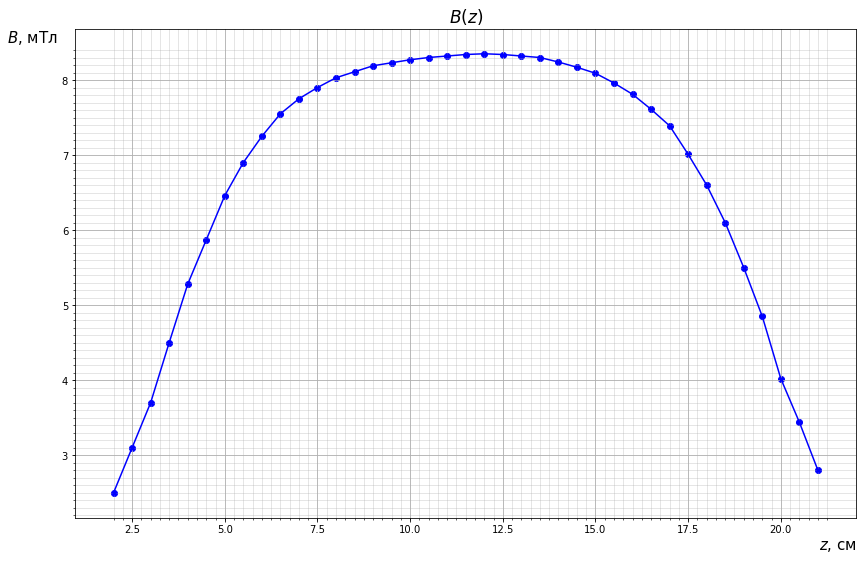
\includegraphics[width=0.7\textwidth]{1_2_ris1.png}
\end{figure}

	3. По графику зависимости $B =B(z)$ определим координату средней точки на оси соленоида (по максимальному значению индукции): $z$ = 12 см.

	4. Установим зонд в среднюю точку на оси соленоида и, изменяя ток через соленоид от $min = 0,5$ A до $max = 2,5$ A, снимем зависимость $B = B(I)$. Полученные данные занесем в таблицу:
    \begin{table}[!htbp]
\centering
	\begin{tabular}{|c|c|c|c|c|c|c|c|c|c|c|c|} \hline
    I, A & 0.5 & 0.6 & 0.7 & 0.8 & 0.9 & 1.0 & 1.1 & 1.2 & 1.3 & 1.4 & 1.5 \\ \hline
    B, мТл & 8.25 & 9.63 & 11.22 & 12.73 & 14.43 & 15.89 & 17.35 & 18.80 & 20.50 & 21.80 & 23.50 \\ \hline
    I, A & 1.6 & 1.7 & 1.8 & 1.9 & 2.0 & 2.1 & 2.2 & 2.3 & 2.4 & 2.5 & \\ \hline
    B, мТл & 24.90 & 26.30 & 28.10 & 29.30 & 30.90 & 32.30 & 33.90 & 35.50 & 36.70 & 38.10 & \\ \hline
	\end{tabular}
\end{table}
    
    
    5. Построим график зависимости $B = B(I)$. Аппроксимирующая прямая $y = 15.0289x + 0.7946$  ($y = kx + c$) найдена с помощью метода наименьших квадратов.
    
    Погрешности: $\sigma_{k} = 0.0447, \sigma_{c} = 0.0271$  
    \begin{figure}[H]
    \centering
	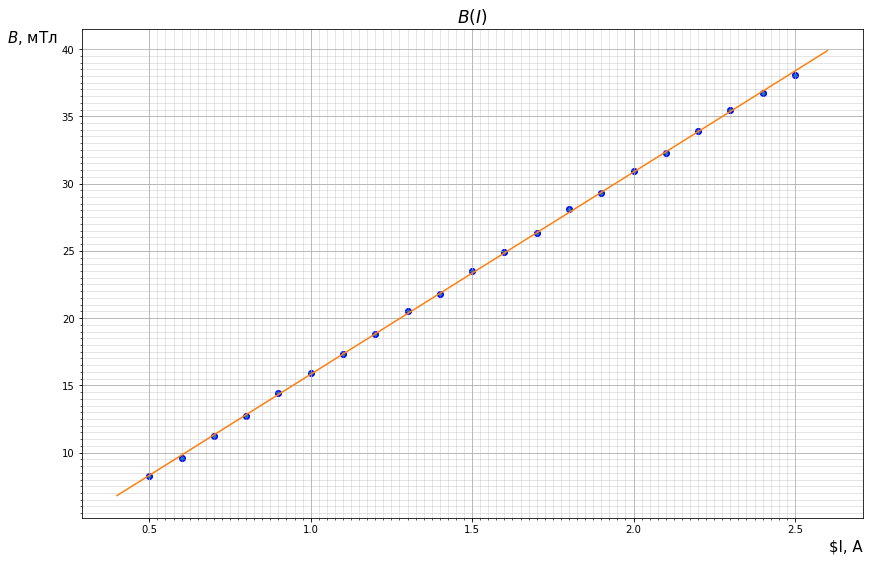
\includegraphics[width=0.8\textwidth]{1_2_ris2.png}
	\end{figure}
	
    6. Теперь оценим длину и диаметр соленоида, полное число витков и плотность намотки соленоида. Исходя из этого, построим теоретическую зависимость поля на оси соленоида.
    Величина магнитного поля на концах соленоида в 2 раза меньше его значения в центре. Тогда крайняя точка имеет координату $z_{k} \approx 3.5$ см, центр z = 12.0 см, тогда длина соленоида равна:
    \[ l = 2(z - z_{k}) = 17 \text{см} = 0.17 \text{м}\]
    
    Теперь найдем плотность намотки $n$, используя график $B = B(I)$.
    Так как в середине длинного соленоида магнитное поле равно:
    \[ B = \mu_{0} n I \]
    (где $\mu_{0} = 1.25663706 \cdot 10^{-6}$ - магнитная постоянная, $n = \frac{N}{l}$ - плотность намотки) то $k = \mu_{0} n $, следовательно,
    \[ n = \frac{k}{\mu_{0}} * 10^{-3} = \frac{15.0289}{1.25663706 \cdot 10^{-6}} \cdot 10^{-3} = 11.9596 \cdot 10^{3}\]
    (на $10^{-3}$ домножаем, так как все результаты записывали в мТл).
    \[ \sigma_{n} = \frac{\sigma_{k}}{\mu_{0}} \cdot 10^{-3} = 35.5713\]
    
    Полное число витков:
    \[ N = ln = 0.17 \cdot (11959.6 \pm 35.6) = 2033.132 \pm 6.052\]
    
    Реальные значения: $l = 24.7$ см, $N = 2300$.

\subsection{Исследование индукции магнитного поля постоянных магнитов}
1. Измерим индукцию магнитного поля в центре постоянного магнита в форме диска. Будем складывать цилиндр из $N$ дисков и измерим зависимость магнитной индукции в центре торца цилиндра от числа магнитов, образующих цилиндр.

\begin{table}[!htbp]
\centering
	\begin{tabular}{|c|c|c|c|c|c|} \hline
    N & 1 & 2 & 3 & 4 & 5  \\ \hline
    B, мТл & 320 & 390 & 420 & 430 & 400  \\ \hline
    N & 6 & 7 & 8 & 8 & 10 \\ \hline
    B, мТл & 390 & 330 & 370 & 390 & 450 \\ \hline
	\end{tabular}
\end{table}

2. Построим график зависимости B(N):
\begin{figure}[H]
\centering
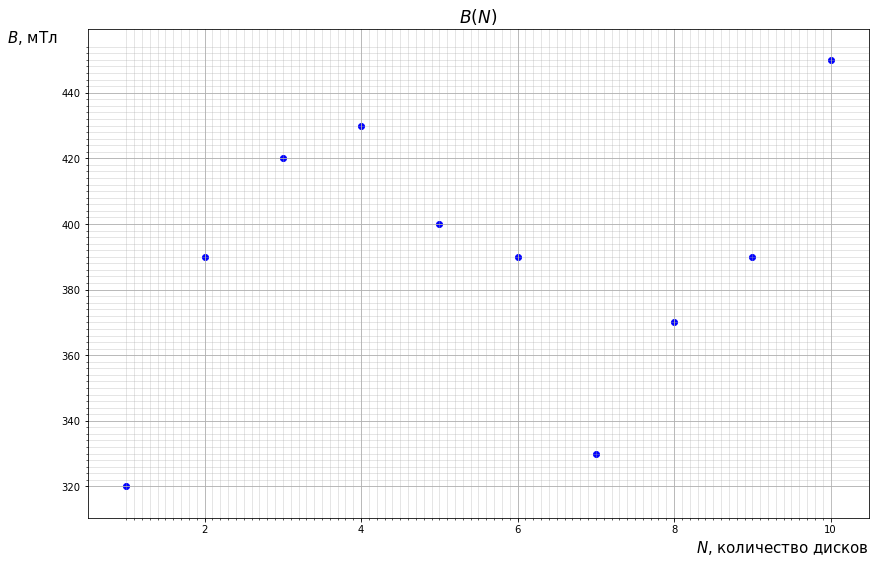
\includegraphics[width=0.8\textwidth]{1_2_ris3.png}
\end{figure}

3. Рассчитаем величину остаточной индукции магнитного поля материала диска. По определению остаточной индукции:
	\[ B_{r}= \mu_{0} p_{m}\]
	С учетом того, что $B = B(h)$:
    \[ B = \frac{1}{2} \mu_{0} p_{m} \frac{h}{\sqrt[2]{r^{2} + h^{2}}}\]
    получаем, что:
    \[ B = \frac{1}{2} B_{r} \frac{h}{\sqrt[2]{r^{2} + h^{2}}}\]

	Для определения остаточной индукции определим угол наклона аппроксимирующей прямой, полученной методом наименьших квадратов из точек зависимости (учитывая, что радиус магнита $r = 0.5$ см, а толщина $d = 0.5$ см.)
	\[ B = B(\frac{1}{2} \frac{h}{\sqrt[2]{r^{2} + h^{2}}})\]
    
    \begin{table}[!htbp]
    	\begin{tabular}{|c|c|c|c|c|c|} \hline
    	$\frac{1}{2} \frac{h}{\sqrt[2]{r^{2} + h^{2}}}$ & 0.3536 & 0.4472 & 0.4743 & 0.4851 & 0.4903 \\ \hline
        B, Тл & 0.32 & 0.39 & 0.42 & 0.43 & 0.40 \\ \hline
        $\frac{1}{2} \frac{h}{\sqrt[2]{r^{2} + h^{2}}}$ & 0.4932 & 0.4949 & 0.4961 & 0.4969 & 0.4975 \\ \hline
        B, Тл & 0.39 & 0.33 & 0.37 & 0.39 & 0.45 \\ \hline
    	\end{tabular}
    \centering
    \end{table}

    \begin{figure}[H]
    \centering
    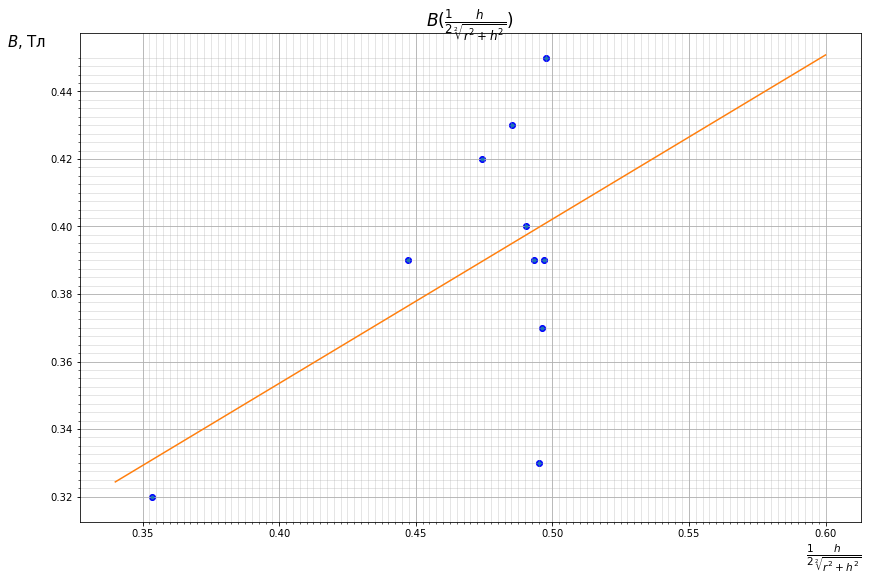
\includegraphics[width=0.8\textwidth]{1_2_ris4.png}
    \end{figure}
    Аппроксимирующая прямая: $y = 0.4865x + 0.1589$  $(y = kx + c)$
    
    Погрешности: $\sigma_{k} = 0.2454, \sigma_{c} = 0.0104$
    
    Получили, что 
    \[ B_{r} = (486.5 \pm 245.4) \text{мТл}\]

	Сравнивая с табличными значениями, и так как погрешность достаточно большая можно предположить, что наш магнит может быть сделан из феррита ($B_{r} = 0.2 - 0.4$ Тл), платины-кобальта ($B_{r} = 0.5$ Тл) или из платины-железа ($B_{r} = 0.6$ Тл).
    
\subsection{Определение намагниченности и остаточной магнитной индукции маленького магнита}

1. Положим между двумя магнитами брусок из бумаги — немагнитного материала. Получим максимальное расстояние, на котором магниты удерживают друг друга в поле тяжести земли:
	\[ r_{max} = 28 \pm 0.05 \text{мм}\]
2. Взвесим оба магнита на весах:
	\[ m_{1} = 2.924 \pm 0.001 \text{г}, m_{2} = 2.956 \pm 0.001 \text{г}\]

3. Рассчитаем величину магнитного момента магнитика $P_{m}$, приравняв силу притяжения двух магнитных диполей $F = \frac{\mu_{0}}{4\pi} 6 P_{m}^{2}/r_{max}^{4}$ силе тяжести $F_{\textbf{т}} = mg$.

	Оценим погрешность расчетов по формуле:
	\[ 4 (\frac{\sigma{P_{m}}}{P_{m}})^{2} =  (\frac{\sigma_{m}}{m})^{2} + (\frac{\sigma_{r_{max}}}{r_{max}})^{2}\]
    
    Отсюда 
   	\[ P_{m} = (17.256 \pm 0.016) \cdot 10^{-2} \text{А * м*м} \]
4. Теперь рассчитаем намагниченность:
	\[ p_{m} = \frac{P_{m}}{V} = (4.39 \pm 0.004) \cdot 10^{5}  \text{А/м} \]
    
    и величину остаточной магнитной индукции:
    \[ B_{r} = \mu_{0} \cdot p_{m} = (552.182 \pm 0.501) \cdot 10^{-3}  \text{Тл}\]
	Значение получилось достаточно похожим и одного порядка со значением, посчитанным в предыдущей части.

\subsection{Определение горизонтальной составляющей магнитного поля Земли}
     \begin{figure}[H]
    \centering
    	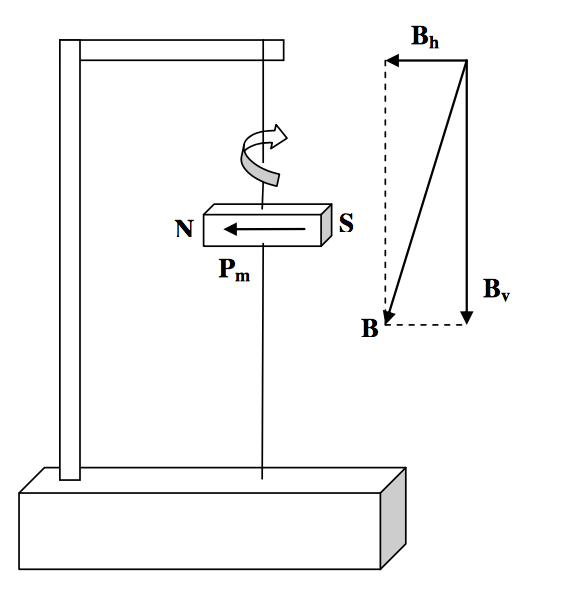
\includegraphics[width=0.2\textwidth]{1_2_ris5.png}
        \caption{Схема установки для измерения горизонтальной составляющей магнитного поля Земли}
    \end{figure}
	1. Возбудим крутильные колебания маятника и определим период его колебаний, измерив время 10 периодов.
	\begin{tabbing}
    \centering
		\begin{tabular}{|c|c|c|c|c|c|} \hline
        $10 T$, c & 19.80 & 19.15 & 19.99 & 19.06 & 19.69 \\ \hline
        $T$, c & 1.980 & 1.915 & 1.999 & 1.906 & 1.969 \\ \hline 
		\end{tabular}
	\end{tabbing}
    $T_{mean} = \frac{\sum T_{i}}{n}$, $\sigma_{T_{mean}} = \sqrt[2]{\frac{1}{n - 1} \sum(T_{i} - T_{mean})^{2}}$
    
    Отсюда получим:
       	\[ T_{mean} = (1.9538 \pm 0.0367) c\]
	2. С помощью штангенциркуля измерим линейные размеры магнита: 
	$b = 4.0 \pm 0.05$ см,
	$a = 1.0 \pm 0.05 $ см.
    
	3. Измерим массу магнита:
	$m = 39.55 \pm 0.001$ г.

	4. По периоду колебаний рассчитаем горизонтальную составляющую магнитного поля Земли $B_{h}$ и оценим погрешность измерений.
	\[ T = 2 \pi \sqrt[2]{\frac{J}{P_{m}}} B_{h}\]
    где
    \[ J = \frac{1}{2} m(a^{2} + b^{2}) = 3.3617 \cdot 10^{-5} \text{кг * м3}\]
    - момент инерции бруска.
    
   \[ B_{h} = \frac{4 \pi^{2} J}{T^{2} P_{m}} =  0.02014 \text{ Тл}\]
   
   Оценим погрешность измерений:
	\[ \sigma_{B_{h}} = 2 (\frac{\sigma_{a}}{a})^{2} + (\frac{\sigma_{m}}{m})^{2} + 2 (\frac{\sigma_{T}}{T})^{2} + (\frac{\sigma_{P_{m}}}{P_{m}})^{2} =  0.00015  \text{ Тл} \]

	Далее, сравним полученные результаты с табличными значениями индукции магнитного поля Земли:
    	\[ B_{h} = 2 \cdot 10^{-5} \text{Тл}\]
        
   По загадочным причинам экспериментальные данные не сошлись с реальными.
\section{Вывод}
	Исследовали зависимости индукции магнитного поля на оси соленоида (от координаты z и от величины тока  I), с помощью чего смогли оценить характеристики соленоида (полное число витков и длину). Исследовали индукции магнитного поля постоянных магнитов. Определили намагниченность и остаточную магнитную индукцию маленького магнита. Определили горизонтальную составляющую магнитного поля Земли.
\end{document}